\documentclass[xetex, hyperref={pdfpagelabels=false}]{beamer}

% --------------------------------------------------------------------------
% Packages
% --------------------------------------------------------------------------
\usepackage[english]{babel}
\usepackage{amsmath, amsthm, amssymb}
\usepackage{bussproofs}
\usepackage{fancyvrb}
\usepackage{geometry}
\usepackage{graphicx}
\usepackage{lmodern}
\usepackage{mylst}
\usepackage{url}


% --------------------------------------------------------------------------
% Tikz Configuration
% --------------------------------------------------------------------------
\usepackage{tikz}
\usetikzlibrary{positioning}
\usetikzlibrary{calc}
\usepackage{rotating}

\tikzset{
    hyperlink node/.style={
        alias=sourcenode,
        append after command={
            let     \p1 = (sourcenode.north west),
                \p2=(sourcenode.south east),
                \n1={\x2-\x1},
                \n2={\y1-\y2} in
            node [inner sep=0pt, outer sep=0pt,anchor=north west,at=(\p1)]
            {\hyperlink{#1}{\XeTeXLinkBox{\phantom{\rule{\n1}{\n2}}}}}
                    %xelatex needs \XeTeXLinkBox, won't create a link unless it
                    %finds text --- rules don't work without \XeTeXLinkBox.
                    %Still builds correctly with pdflatex and lualatex
        }
    }
}
% \usetikzlibrary{shapes.geometric,shapes.symbols,shadows}

\newcommand{\gobackreconstruction}{
  \begin{tikzpicture}[overlay, remember picture, scale=0.5]
    \tikzset{shift={(current page.center)}, xshift=11.7cm,yshift=-8.4cm}
    \node[fill=plum,text=white, hyperlink node = after-reconstruction] (go) at (0,0) {\tiny Go Back};
  \end{tikzpicture}}


% --------------------------------------------------------------------------
% Color definitions.
% --------------------------------------------------------------------------
\usepackage{xcolor}
\definecolor{aliceblue}{rgb}{0.94, 0.97, 1.0}
\definecolor{amber}{rgb}{1.0, 0.75, 0.0}
\definecolor{amethyst}{rgb}{0.6, 0.4, 0.8}
\definecolor{antiquefuchsia}{rgb}{0.57, 0.36, 0.51}
\definecolor{ashgrey}{rgb}{0.7, 0.75, 0.71}
\definecolor{ballblue}{rgb}{0.13, 0.67, 0.8}
\definecolor{blue(munsell)}{rgb}{0.0, 0.5, 0.69}
\definecolor{blue(pigment)}{rgb}{0.2, 0.2, 0.6}
\definecolor{blu}{RGB}{1,0,102}
\definecolor{bondiblue}{rgb}{0.0, 0.58, 0.71}
\definecolor{brightmaroon}{rgb}{0.76, 0.13, 0.28}
\definecolor{cadet}{rgb}{0.33, 0.41, 0.47}

% --------------------------------------------------------------------------
% My palette.
% --------------------------------------------------------------------------
\definecolor{energy}{RGB}{49,247,250}
\definecolor{delicate}{RGB}{67,179,223}
\definecolor{faded}{RGB}{76,117,195}
\definecolor{plum}{RGB}{87,78,164}
\definecolor{petunias}{RGB}{109,80,139}
\definecolor{letour}{RGB}{101,41,105}

% --------------------------------------------------------------------------

% --------------------------------------------------------------------------
% Beamer configuration.
% --------------------------------------------------------------------------
\usetheme{default}
\usecolortheme{default}
\usefonttheme{serif}

\beamertemplatenavigationsymbolsempty
\setbeamertemplate{navigation symbols}{}
\hypersetup{pdfpagemode=UseNone}

% footer.
\setbeamercolor{headFoot}{fg=white, bg=plum!80!black}
\setbeamertemplate{footline}{
  \leavevmode%
  \hbox{%
  \begin{beamercolorbox}
    [wd=.8\paperwidth,ht=2.3ex,dp=1ex,left]{headFoot}%
    \hspace*{2ex}\insertshorttitle\hspace*{2mm}(\insertshortauthor)
  \end{beamercolorbox}%
  \begin{beamercolorbox}
    [wd=.2\paperwidth,ht=2.3ex,dp=1ex,right]{headFoot}%
    \insertframenumber{}/\inserttotalframenumber\hspace*{2ex}
  \end{beamercolorbox}}%
  \vskip 0pt%
  % \vspace*{1mm}%
}

% title in the frame
\setbeamerfont{frametitle}{size=\small,series=\bfseries}
\setbeamercolor{frametitle}{fg=white,bg=plum}

\setbeamerfont{framesubtitle}{size=\normalfont\tiny\itshape}
\setbeamercolor{framesubtitle}{fg=white, bg=plum}

\setbeamercolor{background canvas}{bg=white}
\setbeamercolor{normal text}{fg=black}

% \setbeamercolor{institute}{fg=blu}
\setbeamercolor{title}{fg=plum}
% \setbeamercolor{subtitle}{fg=blu}

% \setbeamercolor{titlelike}{fg=blu}
\setbeamerfont{footnote}{size=\tiny}
\setbeamercolor{footnote}{fg=gray}
% \setbeamercolor{block title}{bg=blue,fg=blu}
% \setbeamercolor{block body}{bg=aliceblue}
% \setbeamercolor{item}{fg=blu} % color of bullets
% \setbeamercolor{subitem}{fg=blu}
% \setbeamercolor{itemize/enumerate subbody}{fg=blu}
% \setbeamertemplate{itemize subitem}{{\textendash}}
% \setbeamerfont{itemize/enumerate subbody}{size=\footnotesize}
% \setbeamerfont{itemize/enumerate subitem}{size=\footnotesize}

% --------------------------------------------------------------------------
% Fonts
% --------------------------------------------------------------------------

\usefonttheme{professionalfonts}
\usefonttheme{serif}
\usepackage{fontspec}
\usepackage{mathtools}
\usepackage{unicode-math}

\setmathfont[ExternalLocation=fonts/
  , BoldFont=xits-mathbold.otf
  ]{xits-math.otf}
\newfontfamily\mathfont{fonts/xits-math.otf}


\setmainfont[ExternalLocation=fonts/
  , BoldFont=SourceSansPro-Semibold.otf
  , BoldItalicFont=SourceSansPro-SemiboldIt.otf
  , ItalicFont=SourceSansPro-It.otf
  ]{SourceSansPro-Regular.otf}

\setmonofont[ExternalLocation=fonts/
  , BoldFont=SourceCodePro-Semibold.ttf
  , BoldItalicFont=SourceCodePro-SemiboldIt.ttf
  , ItalicFont=SourceCodePro-It.ttf
  ]{SourceCodePro-Semibold.ttf}
\newfontfamily\SourceCodeIt{fonts/SourceCodePro-It.ttf}
\newfontfamily\SourceCode{fonts/SourceCodePro-Regular.ttf}

\newcommand{\problemtptp}[3][c]
  {\lstinputlisting[style=tptp,caption=#2, firstline=#3, label=custom#1]{#2}}
\newcommand{\solutiontstp}[2][c]
  {\lstinputlisting[style=tptp,caption=#2, firstline=5, label=custom#1]{#2}}

% --------------------------------------------------------------------------
% References
% --------------------------------------------------------------------------

\usepackage[autostyle]{csquotes}
\usepackage[
    backend=biber
  , style=authoryear-icomp
  , sortlocale=en_US
  , natbib=true
  , url=false
  , doi=true
  , eprint=false
]{biblatex}
\addbibresource{ref.bib}
\renewcommand*{\nameyeardelim}{\addcomma\addspace}
\usepackage{silence}
\WarningFilter{biblatex}{Patching footnotes failed}
\WarningFilter{hyperref}{Token not allowed in a PDF string}

% --------------------------------------------------------------------------
% Title and Author
% --------------------------------------------------------------------------

\title[Proof Reconstruction in Classical Propositional Logic]
  {\textbf{Proof Reconstruction in Classical Propositional Logic}
}
\subtitle{(Work in Progress)}
\date{Agda Implementors’ Meeting XXV\\
May 9-15th}
\author[Jonathan Prieto-Cubides and Andr\'es Sicard-Ram\'irez]{Jonathan Prieto-Cubides\\
(Joint work with Andr\'es Sicard-Ram\'irez)}
\institute{
Universidad EAFIT\\
Medell\'in, Colombia}
% --------------------------------------------------------------------------

\newsavebox\agdapragma

\begin{document}
\setcounter{page}{1}

\begin{frame}[plain]
\titlepage
  \begin{tikzpicture}[overlay, remember picture] (eafit) at (current page.center)
    \node[xshift=0cm,yshift=0cm]
      {
\includegraphics[width=0.25\textwidth]{figures/eafit}};
    \node[xshift=3cm,yshift=-2cm] (chalmers) at (current page.center)
      {
\includegraphics[width=0.25\textwidth]{figures/chalmers}};
  \end{tikzpicture}
\end{frame}


\section{Introduction}

\begin{frame}[fragile, label=reconstruction]{Proof Reconstruction: Overview}

\begin{tikzpicture}
\only<1->{\node(problem) at (0,0)
   {
\includegraphics[scale=0.7]{figures/problem}};
}

\only<2->{\node[right = 0.8cm of problem, hyperlink node=tptp-syntax](tptp){

\includegraphics[scale=0.7]{figures/tptp}
};
}
\only<3->{
\node[right= 0.8cm of tptp, hyperlink node=metis] (metis)
  {
\includegraphics[scale=0.7]{figures/metis}\,
  \footnote{It is available at \url{http://www.gilith.com/software/metis}}
  };
}
\only<4->{
\node[right= 0.8cm of metis, hyperlink node=tstp-syntax] (tstp)
  {
\includegraphics[scale=0.7]{figures/tstp}};
}
\only<5->{
\node[below= 1.5cm of tstp, hyperlink node=athena] (athena)
  {
\includegraphics[scale=0.7]{figures/athena}
  \footnote{It is available at \url{http://github.com/jonaprieto/athena}}
  };
}
\only<6->{
\node[left = 0.5cm of athena, hyperlink node=agda-file] (agdafile)
  {
\includegraphics[scale=0.7]{figures/agdafile}
  };
}
\only<7->{
\node[left = 0.5cm of agdafile, hyperlink node=agda] (agda)
  {
\includegraphics[scale=0.7]{figures/agda}
  \footnote{It is available at \url{http://github.com/agda/agda}}
  };
}
\only<8->{
\node[below = 0.18cm of problem, hyperlink node=verified-example] (verified)
  {
\includegraphics[scale=0.7]{figures/verified}};
}
\only<9->{
\node[below = 0.18cm of verified, opacity=0.5, hyperlink node=failure-example] (failure)
  {
\includegraphics[scale=0.7]{figures/failure}};
}

\only<2->{ \draw[->, thick] (problem) to (tptp)};
\only<3->{ \draw[->, thick] (tptp) to (metis)};
\only<4->{ \draw[->, thick] (metis) to (tstp)};
\only<5->{ \draw[->, thick] (tstp) to (athena)};
\only<6->{ \draw[->, thick] (athena) to (agdafile)};
\only<7->{ \draw[->, thick] (agdafile) to (agda)};
\only<8->{ \draw[->, thick] (agda) to (verified)};
\only<9->{ \draw[->, thick, gray] (agda) to (failure)};
\end{tikzpicture}
\vfill
\end{frame}

\subsection{Motivation}




% \subsection{Proof Reconstruction}

% \subsubsection{Sledgehammer}
% \subsubsection{Waldemesiter}

% \subsection{Automatic Provers}



% \subsubsection{TPTP Syntax}

\begin{frame}{Bonus Slides}
\end{frame}


\begin{frame}[fragile, label=tptp-syntax]{TPTP Syntax}{Thousands of Problems for Theorem Provers}

 \tikz[overlay,remember picture]
  \node at (0.92\textwidth, 0cm)
    {
\includegraphics[width=0.15\textwidth]{figures/tptp}};

  \begin{itemize}
  \item Is a language\footnote{Is available at
        \url{http://www.cs.miami.edu/~tptp/TPTP/SyntaxBNF.html}}
        to encode problems \citep{Sut09}
  \item Is the input of the ATPs
  \item Annotated formulas with the form
   \begin{center}
\begin{tptp}
language(name, role, formula).
\end{tptp}
    \end{center}
    \begin{itemize}
      \item[\texttt{language}] FOF or CNF %THF, TFF,
      \item[\texttt{name}] to identify the formula within the problem
      \item[\texttt{role}] axiom, definition, hypothesis, conjecture, among others
      \item[\texttt{formula}] version in TPTTP format
    \end{itemize}
  \end{itemize}

\gobackreconstruction
\end{frame}

\begin{frame}[fragile, label=tptp-examples]{TPTP Examples}{From Prop-Pack repository
  \footnote{Is available at \url{http://github.com/jonaprieto/prop-pack}}}

\begin{itemize}
  \item $p ⊢ p$
\begin{tptp}
fof(a, axiom, p).
fof(goal, conjecture, p).
\end{tptp}

  \item $⊢ ¬ (p ∧ ¬ p) ∨ (q ∧ ¬ q)$
\begin{tptp}
fof(goal, conjecture, ~ ((p & ~ p) | (q & ~ q))).
\end{tptp}
  \end{itemize}
\gobackreconstruction
\end{frame}

\subsubsection{TSTP Derivations}

\begin{frame}[fragile, label=tstp-syntax]{TSTP Syntax}

 \tikz[overlay,remember picture]
  \node at (0.92\textwidth, -0.5cm)
    {
\includegraphics[width=0.15\textwidth]{figures/tstp}};

A TSTP derivation
\footnote{\url{http://www.cs.miami.edu/~tptp/TPTP/QuickGuide/Derivations.html}}
\begin{itemize}
  \item Is a \hyperlink{tstp-dag}{\textbf{D}irected \textbf{A}cyclic \textbf{G}raph} where
  \begin{itemize}
    \item[\texttt{leaf}] is a formula from the \hyperlink{tptp-syntax}{TPTP} input
    \item[\texttt{node}] is a formula inferred from parent formula
    \item[\texttt{root}] the final derived formula
  \end{itemize}
  \item Is a list of annotated formulas with the form:
  \end{itemize}

\begin{center}
  {\footnotesize
\begin{tptp}
language(name, role, formula, source [,useful info]).
\end{tptp}}
\end{center}

where \textbf{source} typically is an inference record:
\begin{center}
{\footnotesize
\begin{tptp}
inference(rule, useful info, parents)
\end{tptp}
}
\end{center}
\gobackreconstruction
\end{frame}

\begin{frame}[fragile, label=tstp-example]{TSTP Example}

 \tikz[overlay,remember picture]
  \node at (0.93\textwidth, -0.3cm)
    {
\includegraphics[width=0.15\textwidth]{figures/metis}};

\begin{itemize}
  \item Proof found by \texttt{Metis} ATP for the problem $p ⊢ p$
{\small
\begin{tptp}
$ metis --show proof basic-4.tptp
fof(a, axiom, (p)).
fof(goal, conjecture, (p)).
fof(subgoal_0, plain, (p),
  inference(strip, [], [goal])).
fof(negate_0_0, plain, (~ p),
  inference(negate, [], [subgoal_0])).
fof(normalize_0_0, plain, (~ p),
  inference(canonicalize, [], [negate_0_0])).
fof(normalize_0_1, plain, (p),
  inference(canonicalize, [], [a])).
fof(normalize_0_2, plain, ($false),
  inference(simplify, [],
    [normalize_0_0, normalize_0_1])).
cnf(refute_0_0, plain, ($false),
    inference(canonicalize, [], [normalize_0_2])).
\end{tptp}
}
\end{itemize}
\gobackreconstruction
\end{frame}


\begin{frame}[fragile, label=tstp-dag]{DAG for the previous TSTP derivation found by \texttt{Metis} ATP}

\vfill
\begin{center}
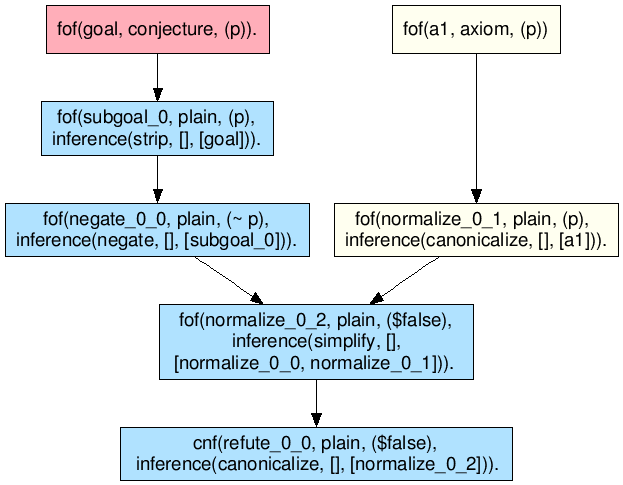
\includegraphics[height=0.8\textheight]{figures/derivation.png}
\end{center}
\gobackreconstruction
\end{frame}


\begin{frame}[fragile, label=athena]{Athena}
 \tikz[overlay,remember picture]
  \node at (0.92\textwidth, 1cm)
    {
\includegraphics[width=0.15\textwidth]{figures/athena}};
\begin{block}{Athena} Is a Haskell program that translates proofs given by Metis Prover
in TSTP format to Agda code.\\
It depends on:
\begin{itemize}
  \item \texttt{agda-prop} Classical Logic within Agda: Axioms + Theorems
  \item \texttt{agda-metis} Theorems of the inference rules of Metis Prover
\end{itemize}
\end{block}
\gobackreconstruction
\end{frame}


\begin{frame}[label=haskell]{Design Decisions for the Reconstruction Tool}
 \tikz[overlay,remember picture]
  \node at (0.93\textwidth, 0cm)
    {
\includegraphics[width=0.2\textwidth]{figures/athena}};

\begin{block}{Haskell} % is a standardized, general-purpose purely functional programming language.\\ Our usages:
\begin{itemize}
    \item Parsing
    \item AST construction
    \item Creation and analysis of \hyperlink{tstp-dag}{DAG} derivations
    \item Analysis of inference rules used
    \item Generation of Agda code of the proof
\end{itemize}
\end{block}
\gobackreconstruction
\end{frame}

\begin{frame}[label=agda]{Design Decisions for the Reconstruction Tool}{Programming Languages}

 \tikz[overlay,remember picture]
  \node at (0.92\textwidth, 1cm)
    {
\includegraphics[width=0.15\textwidth]{figures/agda}};

\begin{block}{Agda}
Is a dependently typed functional programming language and it also a proof assistant.\\
We used it to type-check the proofs found by Metis Prover
    \begin{itemize}
    \item Agda-Prop Libary: Logic framework for Classical Propositional Logic
    \item Agda-Metis Library: theorems based on the inference rules of Metis Prover
    \end{itemize}
\end{block}
\gobackreconstruction
\end{frame}

\begin{frame}[label=metis]{Metis Theorem Prover}{\url{http://www.gilith.com/software/metis/}}
 \tikz[overlay,remember picture]
  \node at (0.92\textwidth, 0.5cm)
    {
\includegraphics[width=0.15\textwidth]{figures/metis}};

Metis is an automatic theorem prover for First-Order Logic with equality
\begin{block}{Why Metis?}
  \begin{itemize}
    \item \href{https://github.com/gilith/metis}{Open source} implemented in Standard ML
    \item Reads problem in \hyperlink{tptp-syntax}{\texttt{TPTP} format}
    \item Outputs detailed proofs in \hyperlink{tstp-format}{\texttt{TSTP} format}
    \item Each refutation step is one of
      \href{http://www.gilith.com/software/metis/logical-kernel.txt}{\textbf{6 simple rules}}
  \end{itemize}
\end{block}
\gobackreconstruction
\end{frame}


\begin{frame}[fragile, label=metis-rules]{Inference Rules of Metis}
\hyperlink{tstp-example}{TSTP} derivations exhibit these inferences:
\vfill
\begin{table}[!ht]
\begin{center}
\scalebox{0.8}{
{\renewcommand{\arraystretch}{1.3}%
\begin{tabular}{|cl| }
\hline
\textbf{Rule} & \textbf{Task} \\
\hline
\texttt{canonicalize} & transforms formulas to CNF, DNF or NNF\\
\texttt{clausify} & performs clausification\\
\hyperlink{atp-conjunct}{\texttt{conjunct}} & extracts a formula from a conjunction\\
\texttt{negate} & applies negation to the formula\\
\texttt{resolve} & applies theorems of resolution\\
\texttt{simplify} & applies over a list of formula to simplify them\\
\texttt{strip} & splits a formula into subgoals\\[1ex]
\hline
\end{tabular}}
}
\end{center}
\label{tab:label}
\end{table}
\vfill
\gobackreconstruction
\end{frame}


\begin{frame}[fragile, label=atp-conjunct]{Conjunct}{Inference Rule}
\begin{block}{conjunct}
\begin{agda}
conjunct : Prop → Prop → Prop
conjunct (φ ∧ ψ) ω with ⌊ eq φ ω ⌋ | ⌊ eq ψ ω ⌋
... | true  | _     = φ
... | false | true  = ψ
... | false | false = conjunct φ ω
conjunct φ ω        = φ

atp-conjunct
  : ∀ {Γ} {φ}
  → (ω : Prop)
  → Γ ⊢ φ
  → Γ ⊢ conjunct φ ω
\end{agda}
\end{block}
\end{frame}


\begin{frame}[fragile, label=agda-file]{Agda Code}{Generated by Athena Tool}
Example goes here
\gobackreconstruction
\end{frame}

\begin{frame}[fragile, label=verified-example]{Type-checked Proof}
Verified Example goes here
\gobackreconstruction
\end{frame}

\begin{frame}[fragile, label=failure-example]{Type-checked Proof}
Failure Example goes here
\gobackreconstruction
\end{frame}


\begin{frame}[fragile, label=hammer]{Related Work}
\begin{block}{SledgeHammer}
\begin{itemize}
\item Isabelle/HOL tool
\item Metis ported within Isabelle
\item Reconstruct proofs of well-known ATPs: EProver, Vampire, among others
\end{itemize}
\end{block}

\begin{block}{Integrating Waldmeister and Agda}
\begin{itemize}
  \item Source code not available
  \item Equational Logic
  \item Reflection Layers
  \end{itemize}
\end{block}
\end{frame}


\begin{lrbox}{\agdapragma}
\begin{agda}
module Or where

data _OR_ (A B : Set) : Set where
  inj1 : A → A OR B
  inj2 : B → A OR B

postulate
  A B    : Set
  OR-comm : A OR B → B OR A
{-# ATP prove OR-comm #-}
\end{agda}
\end{lrbox}

\begin{frame}[fragile, label=after-reconstruction]
\end{frame}

\begin{frame}[fragile]{Related Work: Apia}
  {Proving first-order theorems written in Agda using automatic theorem provers for first-order logic}

\only<1-2>{At the moment, the communication between Agda and
the ATPs is unidirectional because the ATPs are being used as oracles \citep{Sicard2015}.}
\only<1-2>{\vfill}


\begin{tikzpicture}
\only<1->{ \node(agdafile) at (0,0){
  
\includegraphics[scale=0.8]{figures/agda-pragmas}}};
\only<1>{
  \node[fill=aliceblue, rectangle, right = 2.5cm of agdafile] (atp-pragmas){
  \scalebox{0.7}{\usebox\agdapragma}
  }
  };


\only<2->{
  \node[right=1cm of agdafile] (eagda){
  
\includegraphics[scale=0.8]{figures/eagda}
  \footnote{Development version of Agda in order to handle a new built-in ATP-pragma.
    \url{https://github.com/asr/eagda}}
  }
};

\only<2->{
\node[right=1cm of eagda] (agdai){
  
\includegraphics[scale=0.8]{figures/agdai}
  }
};

\only<3->{
  \node[below=0.4cm of agdai] (apia){
  
\includegraphics[scale=0.8]{figures/apia}
  \footnote{Haskell program for proving first-order theorems written in Agda using ATPs.
    \url{https://github.com/asr/apia}}}
  };

\only<4->{
  \node[left= 1cm of apia] (tptp)
    {
\includegraphics[scale=0.8]{figures/tptp}}};

\only<5->{ \node[below = 0.8cm of apia] (atp)
  {
\includegraphics[scale=0.8]{figures/atp}}};

\only<7->{ \node[below = 2.4 of agdafile, rectangle, text=white,fill=black, align=left, font=\tiny] (proved)
{
\texttt{\$ agda Or.agda}\\
\texttt{\$ apia Or.agda --atp=online-metis}\\
\texttt{Metis---2.3 proved the conjecture}
  }
};

\only<2->{\draw[->, ultra thick] (agdafile) to (eagda)};
\only<2->{\draw[->, ultra thick] (eagda) to (agdai)};
\only<3->{\draw[->, ultra thick] (agdai) to (apia)};
\only<4->{\draw[->, very thick, dashed, gray] (apia) to (tptp)};
\only<5->{\draw[->, very thick, dashed, gray] (tptp) to (atp)};
\only<6->{\draw[->, very thick, dashed, gray] (atp) to (apia)};

\end{tikzpicture}
\end{frame}


\begin{frame}[label=future-work]{Future Work}
\begin{itemize}
  \item Add shallow embedding in order to work with \texttt{Apia}
  \item Support First-Order Logic with Equality
  \item Support another prover like \texttt{EProver}\textbf{
}\end{itemize}
\end{frame}


\begin{frame}[label=references]{References}
\printbibliography
\end{frame}



\end{document}